\chapter{Planned schedule} \label{ch-schedule}
Below is a Gantt chart indicating our proposed research milestones and timeline. Uncertainty quantification work for the first objective is complete, and a journal article for submission in the \textit{Journal of Quantitative Spectroscopy and Radiative Transfer} (JQSRT) is in progress. It is in collaboration with two authors from Sandia National Laboratories, requiring an additional review and approval (R\&A) process. We intend to submit to R\&A by mid-February, and submit to JQSRT as soon as that process is complete. 
Work on the second objective, global sensitivity analysis, began with investigating the Saltelli approach as part of a submitted transactions for ANS Winter 2022. We also submitted an extended abstract on GSA to M\&C 2023, and next steps are to extend that work into a full journal article. Objective two research work is approximately 30\% complete with the beginning investigations into the Saltelli approach. 
Work on the third objective, the challenge problem and increased complexity, is underway as we have started integrating variance deconvolution UQ into MC/DC.

\begin{figure}[ht]
    \centering
    \centerline{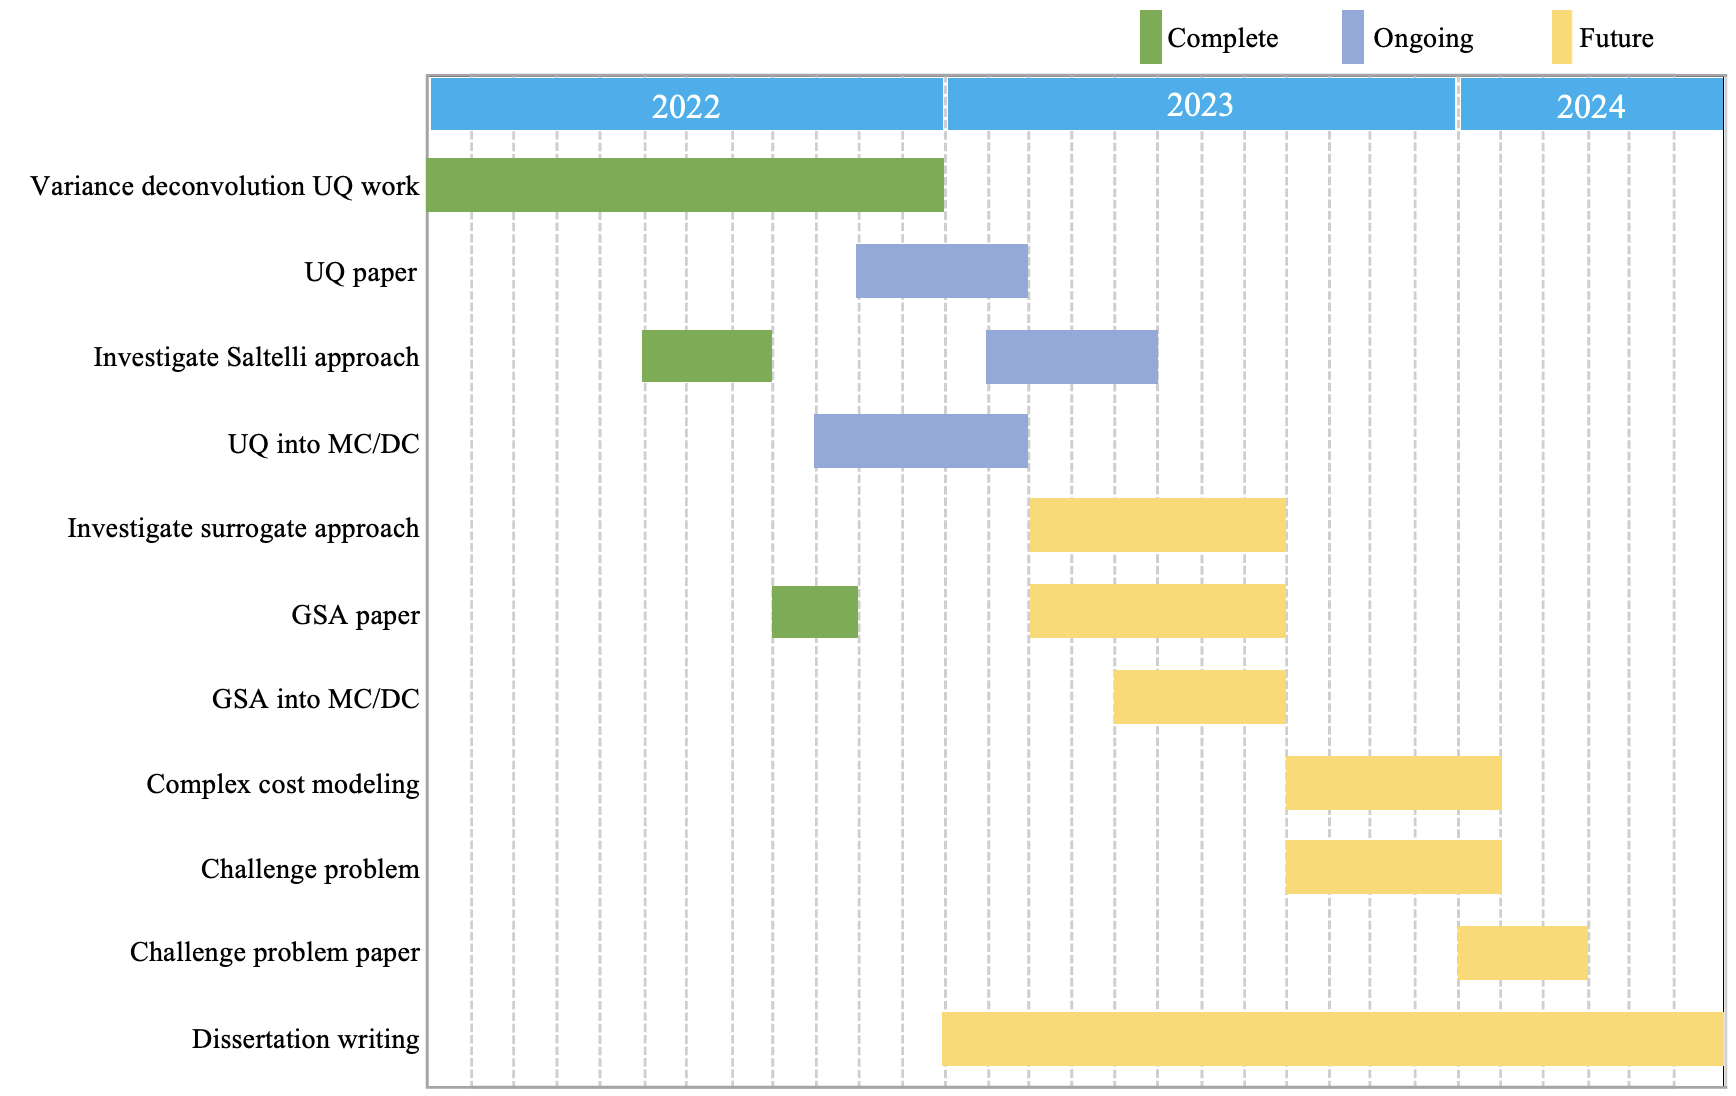
\includegraphics[scale=0.5]{Figures/gantt-third.png}}
    \label{fig:gantt}
\end{figure}
